\chapter{Grundlagen}
\label{ch:grundlagen}

	\section{Netzwerke}
	\label{sec:grundlagen:netzwerke}
	
	Ein Computernetzwerk besteht mindestens aus zwei Computern, einem Übertragungsmedium und Protokollen, die festlegen, in welcher Form die Computer Daten austauschen Ein Computernetz kann sich physisch über einige Meter (dann spricht man von einem \ac{PAN}) bis über die gesamte Erde (dann spricht man von einem \ac{GAN}) ausdehnen. Das Internet ist ein GAN. \cite{Baun2018-A}.\\
	
	Beim \ac{OSI} Referenzmodell (vgl. Abbildung \ref{fig:grundlagen:osi}) wird eine Netzwerkverbindung in sieben logische Schichten unterteilt. Es wird verwendet, um eine Kommunikation über ein Netzwerk darzustellen. Die einzelnen Schichten sind dabei durch Schnittstellen miteinander verbunden, sodass einzelne Protokolle leicht ausgetauscht werden können \cite{Baun2018-B}
	
	\begin{figure}[htbp]
		\centering
		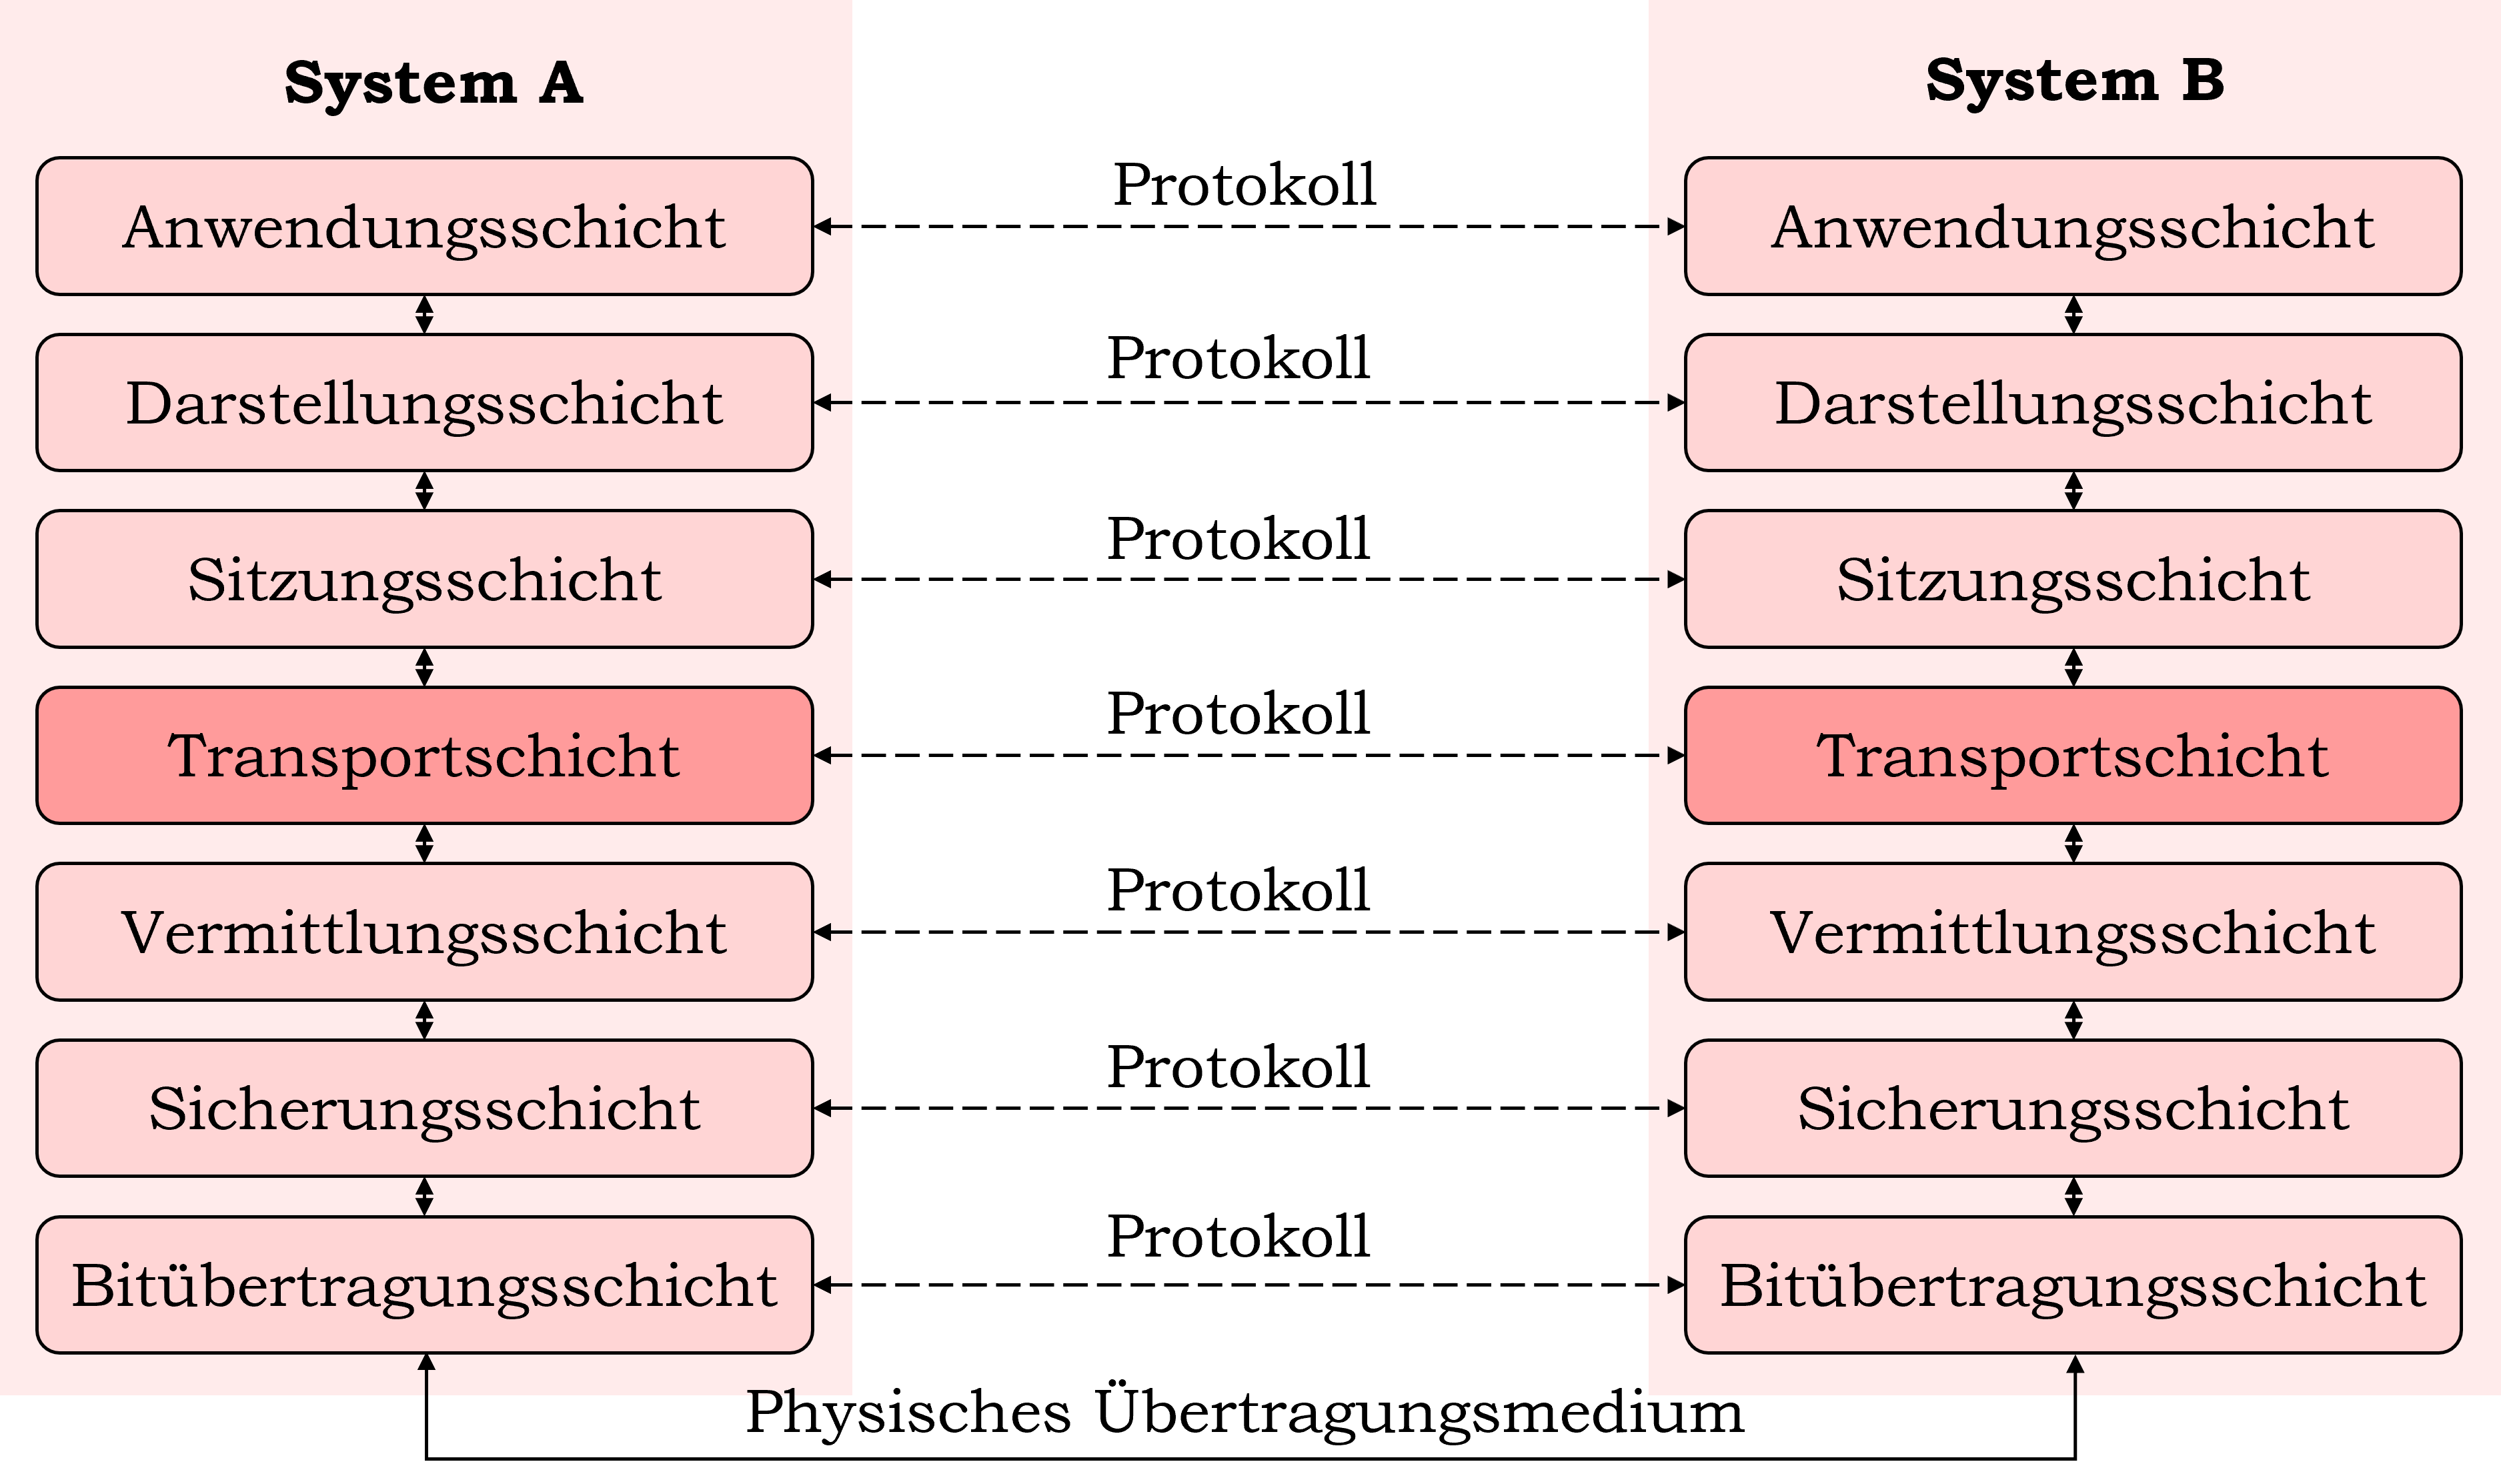
\includegraphics[width=\textwidth]{chapters/abb/grundlagen-osi}
		\caption{OSI-Referenzmodell mit hervorgehobener Transportschicht}
		\label{fig:grundlagen:osi}
	\end{figure}

	\section{Kryptographie}
	\label{sec:grundlagen:krypto}
	
	Der Begriff Kryptographie bezeichnet die ''Wissenschaft vom geheimen Schreiben'' \cite{Waetjen2018}. Dabei wird der verschlüsselte Text als ''Chiffretext'' und der entschlüsselte Text als ''Klartext'' bezeichnet. Das Gegenstück der Kryptographie ist die Kryptanalyse, deren Ziel es ist, Kryptographie zu brechen. Kryptographie und Kryptanalyse bilden das Fachgebiet der Kryptologie \cite{Paar2010}.
	
	Ein wichtiges Prinzip der Kryptographie ist das Kerckhoffsche Prinzip. Dieses besagt, dass die verwendeten Methoden zur Ver- und Entschlüsselung auch dann noch sicher sein müssen, wenn sie öffentlich bekannt sind. Dies bedeutet, dass die Sicherheit des Verfahrens auf dem Schlüssel basieren muss.\\
	
	Dies ist aus mehreren Gründen entscheidend. Zum einen ist es i. d. R. nicht oder nur mit großen Schwierigkeiten möglich, ein gesamtes Verfahren unter Verschluss zu halten. Die Geheimhaltung eines Schlüssels ist deutlich einfacher. Zum anderen ist es so möglich, das Verfahren durch Dritte evaluieren zu lassen und auf Fehler hingewiesen werden zu können \cite{Kuesters2011-A}.\\
	
	Innerhalb der Kryptographie unterscheidet man dann zwischen symmetrischer und asymmetrischer Kryptographie \cite{Paar2010}. Diese werden im Folgenden näher betrachtet.
	
		\subsection{Symmetrische Kryptographie}
		\label{subsec:grundlagen:krypto:sym}
		
		Bis 1976 wurde ausschließlich mit symmetrischer Kryptographie gearbeitet. Klassische Einsatzgebiete dieser Art der Verschlüsselung sind auch heute noch die Datenverschlüsselung sowie Integritätsprüfungen.\\
		
		Bei der symmetrischen Kryptographie werden für die Ver- und Entschlüsselung der gleiche Schlüssel verwendet. Der zu verschlüsselnde Klartext wird mit dem Schlüssel verschlüsselt und kann dann über einen unsicheren Kanal transportiert werden. Der Empfänger erhält den Chiffretext und kann diesen mithilfe des gleichen Schlüssels wieder in den Klartext umwandeln.\\
		
		Ein großes Problem dieser Art der Verschlüsselung ist das Problem des sicheren Schlüsselaustauschs. Die beiden Kommunikationspartner müssen sich auf einen Schlüssel einigen. Dies muss jedoch über einen sicheren Kanal geschehen, damit sichergestellt werden kann, dass der Schlüssel nicht an unberechtigte Dritte gerät \cite{Paar2010}.\\
		
		Innerhalb der symmetrischen Kryptographie kommen Strom- und Blockchiffren zum Einsatz. Während Stromchiffren jedes Bit des Klartexts einzeln verschlüsseln, verschlüsseln Blockchiffren den Klartext in Blöcken fester Größe \cite{Paar2010-B}.\\
		
		Stromchiffren sind besonders für Echtzeitanwendungen und für den Einsatz auf Systemen mit begrenzten Ressourcen geeignet. Dies liegt daran, dass sie hereinkommende Bits sofort verschlüsseln und über einen unsicheren Kanal übertragen können. Sie sind nicht darauf angewiesen, eine bestimmte Menge an Daten abzuwarten. Eine bekannte Stromchiffren ist beispielsweise RC4, die bei HTTPS zum Einsatz kommt.\\
		
		In den meisten Anwendungen, in denen symmetrische Kryprographie zum Einsatz kommt, werden jedoch Blockchiffren verwendet \cite{Paar2010-B}. Auf Blockchiffren bauen viele weitere Bausteine der Kryptographie auf. So können beispielsweise Stromchiffren oder Hashfunktionen durch Blockchiffren erzeugt werden.
		
		\subsection{Asymmetrische Verschlüsselung}
		\label{subsec:grundlagen:krypto:asym}
		
		Im Gegensatz zur symmetrischen Kryptographie wird bei der asymmetrischen Kryptographie nicht derselbe Schlüssel für Ver- und Entschlüsselung verwendet. Der Grundgedanke ist, dass der Schlüssel für die Entschlüsselung geheim gehalten werden muss, der Schlüssel für die Verschlüsselung jedoch nicht.\\
		
		\begin{figure}[htbp]
			\centering
			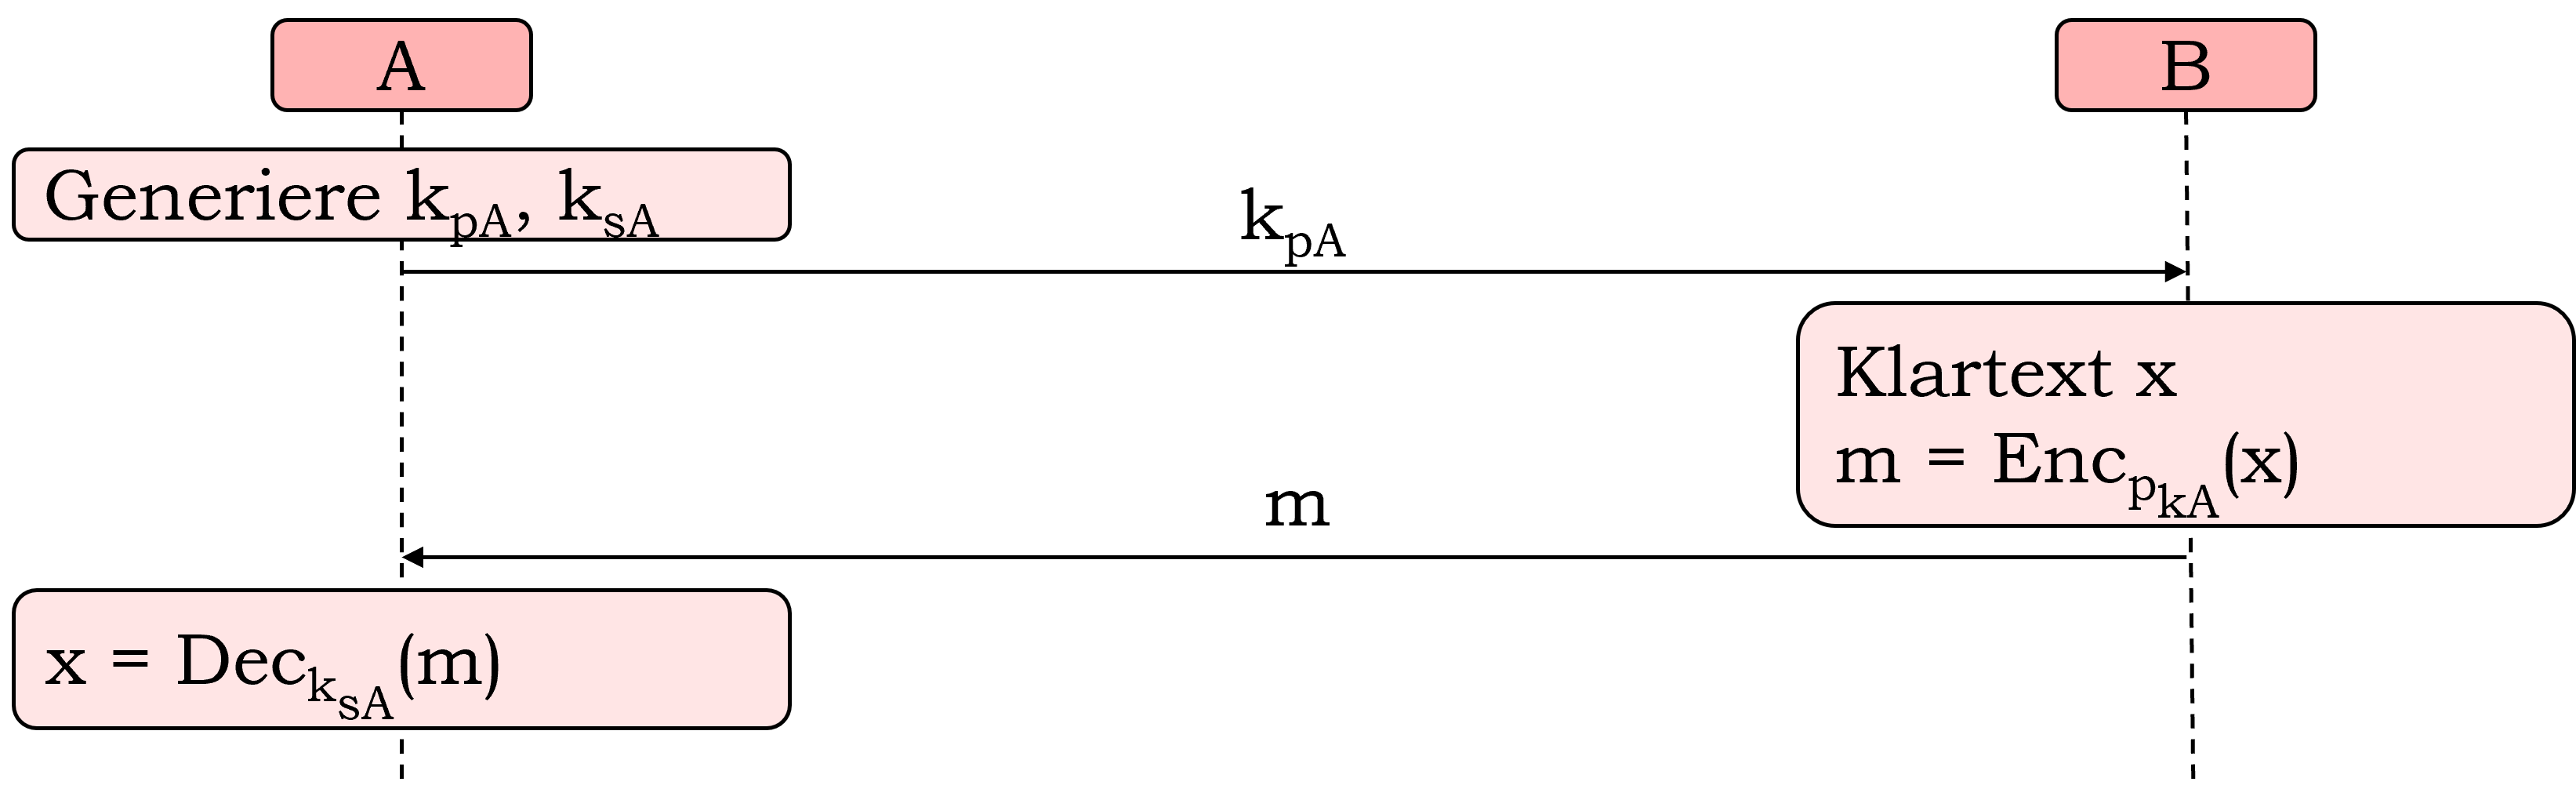
\includegraphics[width=\textwidth]{chapters/abb/grundlagen-krypto-asym}
			\caption{Ein einfaches asymmetrisches kryptographisches Verfahren}
			\label{fig:krypto:asym}
		\end{figure}
		
		Asymmetrische kryptographische Verfahren basieren jeweils auf einem von drei mathematischen Problemene:
		
		\begin{enumerate}
			\item Primfaktorzerlegung
			\item Diskreter Logarithmus
			\item Elliptische Kurven
		\end{enumerate}
	
		Alle diese Probleme haben gemein, dass sie ohne Zusatzinformationen nur mit einem sehr großen Zeitaufwand durch einen Computer gelöst werden können. Die Zusatzinformation, die das Lösen des Problems und somit das Entschlüsseln der Nachricht ermöglicht, ist der private Schlüssel des Empfängers der Nachricht \cite{Paar2010-C}.
		
		Ein bekanntes Beispiel für eine asymmetrische Chiffre, die auf dem mathematischen Problem der Primfaktorzerlegung basiert, ist \ac{RSA} (vgl. Abschnitt \ref{subsubsec:grundlagen:krypto:auth:rsa}.\\
		
		Der diskrete Logarithmus ist beispielsweise Grundlage des Diffie-Hellman-Schlüsselaustauschs \ref{fig:grundlagen:dhke}. Für diesen gibt es auch eine Variante, die elliptische Kurven verwendet.\\
		
		\begin{figure}[htbp]
			\centering
			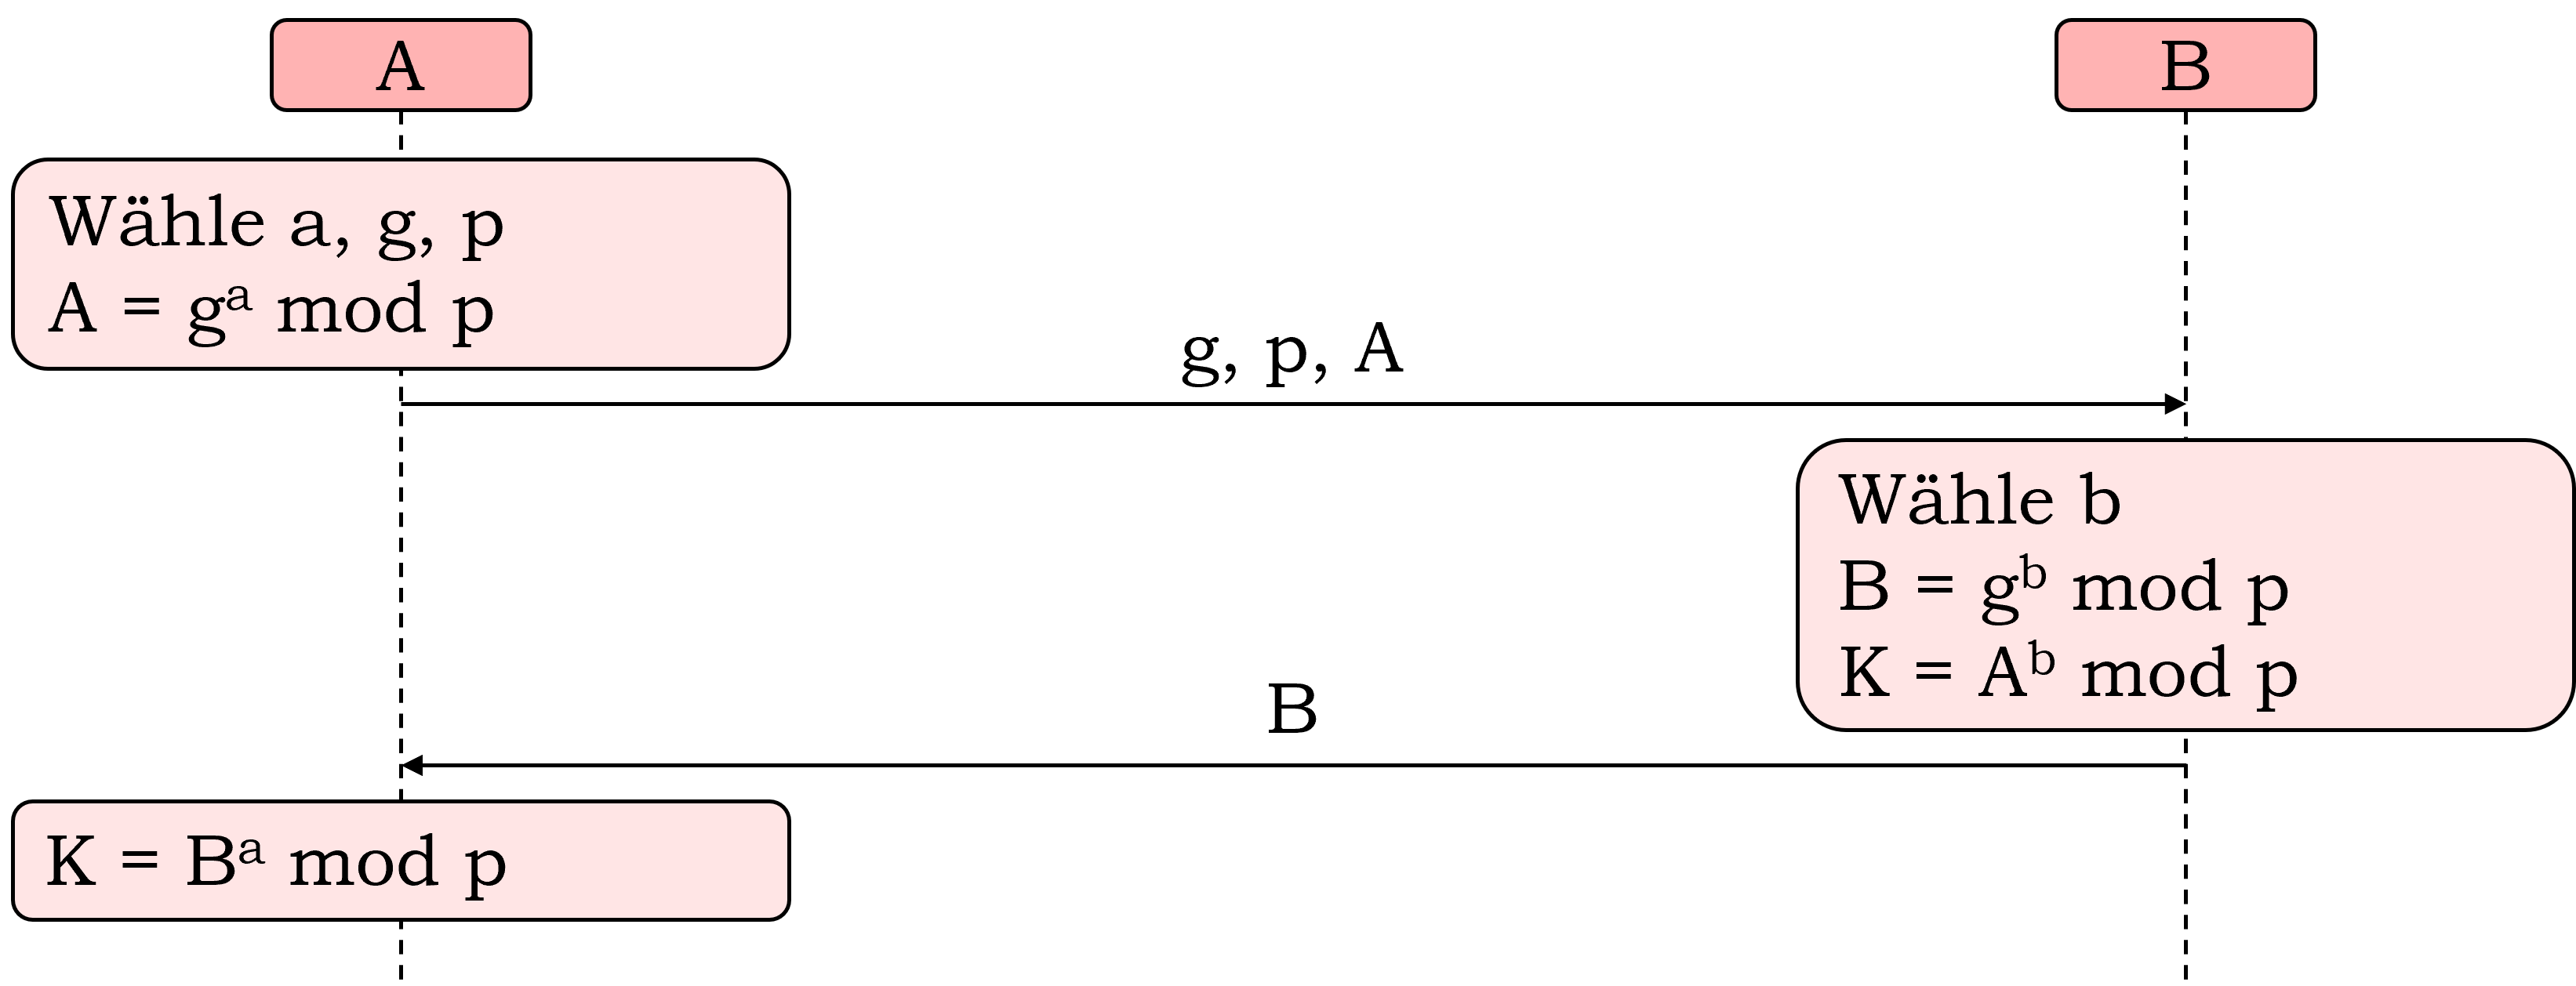
\includegraphics[width=\textwidth]{chapters/abb/grundlagen-dhke}
			\caption{Funktionsweise des Diggie-Hellman-Schlüsselaustauschs}
			\label{fig:grundlagen:dhke}
		\end{figure}
		
		\subsection{Kryptographische Hashfunktionen}
		\label{subsec:grundlagen:krypto:hash}
		
		Hashfunktionen sind kryptographische Funktionen, die eine Eingabe beliebiger Länge auf eine Ausgabe fester Länge abbildet. Diese Berechnung muss sehr einfach erfolgen können. Auf der Ausgabe können jedoch keine Schlüssel auf die Eingabe geschlossen werden.\\
		
		Weiterhin darf zu einem bekannten Eingabewert keine zweite Eingabe gefunden werden können, die den gleichen Hashwert ergibt. Diese Eigenschaft bezeichnet man als schwache Kollisionsresistenz.\\
		
		Außerdem gibt es die starke Kollisionsresistenz. Diese besagt, dass keine frei wählbare unterschiedlichen Eingaben gefunden werden dürfen, die den gleichen Hashwert ergeben.\\
		
		Hashfunktionen können entweder eine eigene designierte Hashfunktion sein oder auf einer symmetrischen Blockchiffre basieren. Designierte Hashfunktionen sind beispielsweise \ac{SHA}-2 und SHA-3.
		
		\subsection{Authentifizierungsverfahren}
		\label{subsec:grundlagen:krypto:auth}
		
		Auch bei den Authentifizierungsverfahren unterscheidet man zwischen symmetrischen Verfahren und asymmetrischen Verfahren. Auch diese sollen im folgenden genauer betrachtet werden.
		
			\subsubsection{Symmetrische Authentifizierungsverfahren}
			\label{subsubsec:grundlagen:krypto:auth:sym}
			
			Symmetrische Authentifizierungsverfahren werden auch als \Ac{MAC} bezeichnet. Sie basieren in der Regel auf Blockchiffren (vgl. Abschnitt \ref{subsec:grundlagen:krypto:sym}) oder kryptographischen Hashfunktionen (vgl. Abschnitt \ref{subsec:grundlagen:krypto:hash}) \cite{Kuesters2011-B}.\\
			
			MACs generieren aus einer Nachricht beliebiger Länge eine kryptographische Prüfsumme, die unabhängig von der Länge der Nachricht immer die gleiche Länge hat. Da es sich hier um ein symmetrisches Verfahren handelt, benötigen die Kommunikationspartner einen gemeinsamen kryptographischen Schlüssel.\\
			
			Die Prüfsumme erlaubt es, Manipulationen an der Nachricht zu erkennen sowie den Ursprung der Nachricht nachzuvollziehen. Mit MACs ist es jedoch nicht möglich, die Urheberschaft einer Nachricht eindeutig einer Person zuzuordnen. Es kann lediglich festgestellt werden, dass die Person den Schlüssel kennt. Diesen kennen jedoch immer mindestens zwei Parteien.\\
			
			MACs können auf Blockchiffren basieren. Häufig wird beispielsweise AES im \ac{CBC} Modus dafür verwendet. Dafür werden für die einzelnen Blöcke der zu authentifizierenden Nachricht die folgenden Berechnungen durchgeführt:
			
			\[ y_{1} = Enc_{k}(x_{1} \oplus IV) \]
			\[ y_{2} = Enc_{k}(x_{2} \oplus y_{1}) \]
			\[ y_{i} = Enc_{k}(x_{i} \oplus y_{i-1}) \]
			
			Ein einfaches Verfahren für einen MAC, der auf einer Hashfunktion basiert, ist der HMAC. In der Abbildung wird der Schlüssel als geheimer Präfix verwendet. Dieser könnte jedoch auch als Suffix verwendet werden. \cite{Paar2010-D}\\ 
			
			\begin{figure}[htbp]
				\centering
				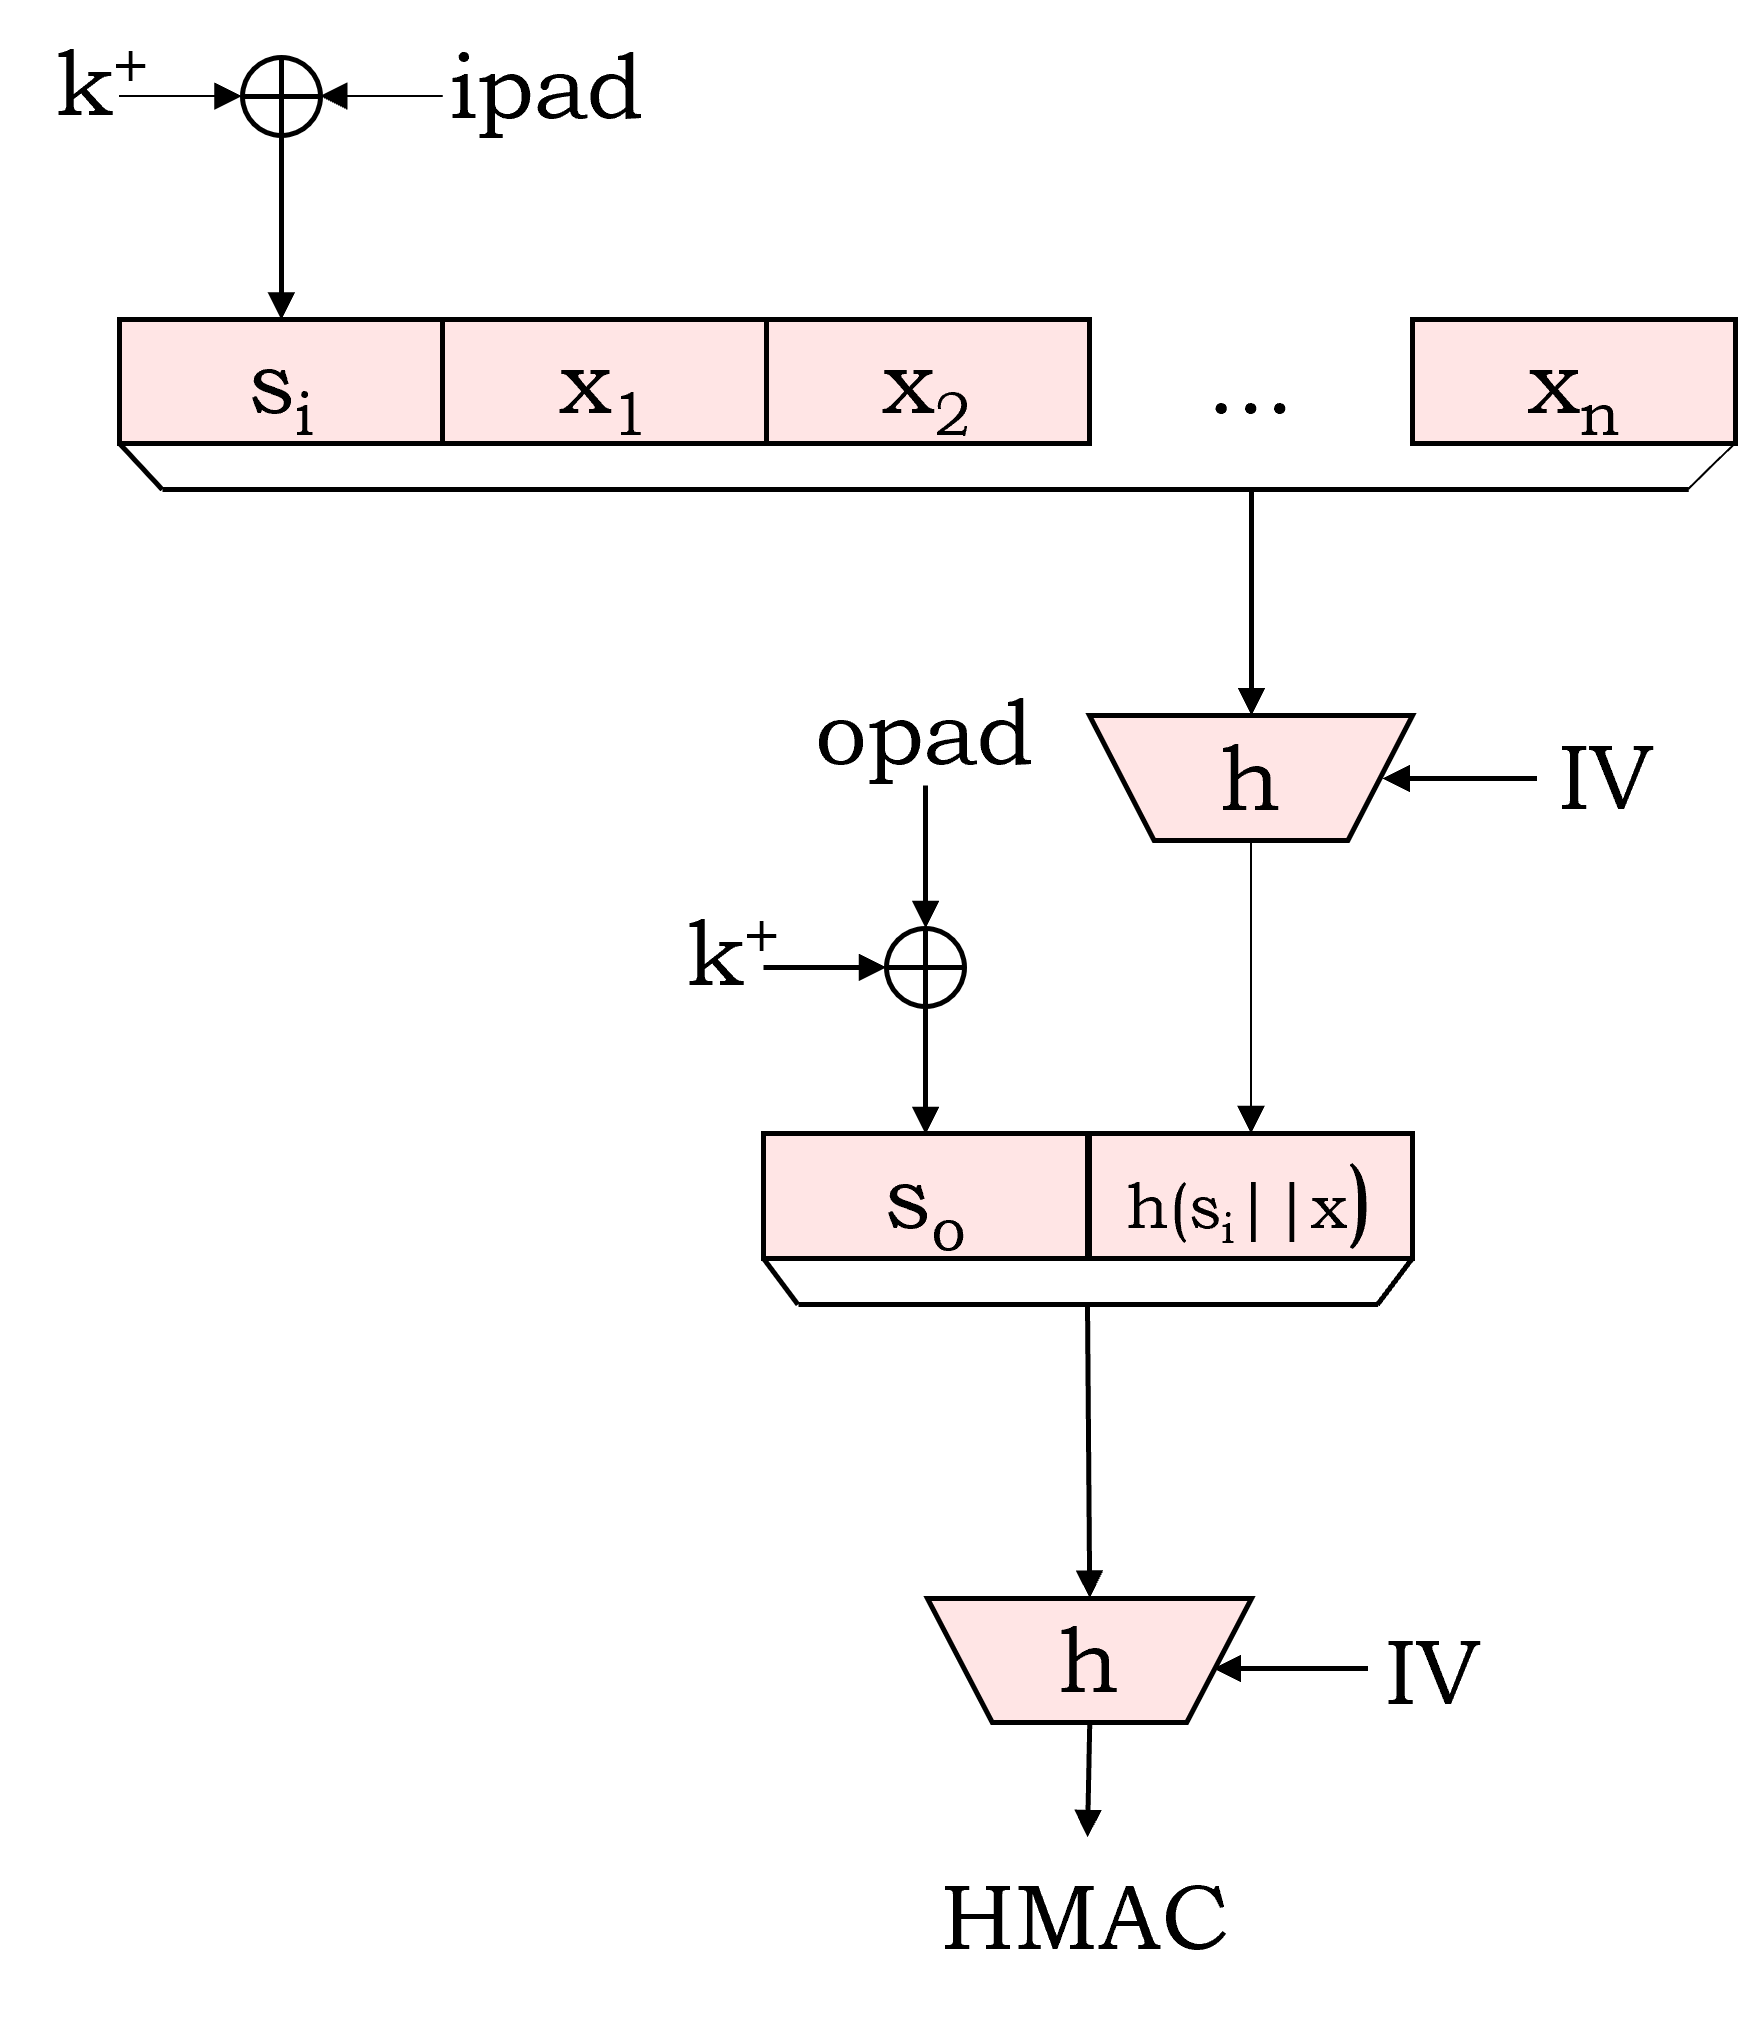
\includegraphics[width=\textwidth]{chapters/abb/grundlagen-hmac}
				\caption{Ein einfaches HMAC-Verfahren}
				\label{fig:grundlagen:hmac}
			\end{figure}
			
			\subsubsection{Asymmetrische Authentifizierungsverfahren}
			\label{subsubsec:grundlagen:krypto:auth:asym}
			
			Asymmetrische Authentifizierungsverfahren werden auch als Digitale Signaturen bezeichnet. Dabei verschlüsselt die zu authentifizierende Partei einen Klartext mit ihrem privaten Schlüssel und schickt den Klartext und den Chiffretext an den Kommunikationspartner. Wenn dieser den Chiffretext mit dem öffentlichen Schlüssel der zu authentifizierenden Person entschlüsselt und den korrekten Klartext erhält, ist die Authentifizierung erfolgreich verlaufen.\\
			
			\begin{figure}[htbp]
				\centering
				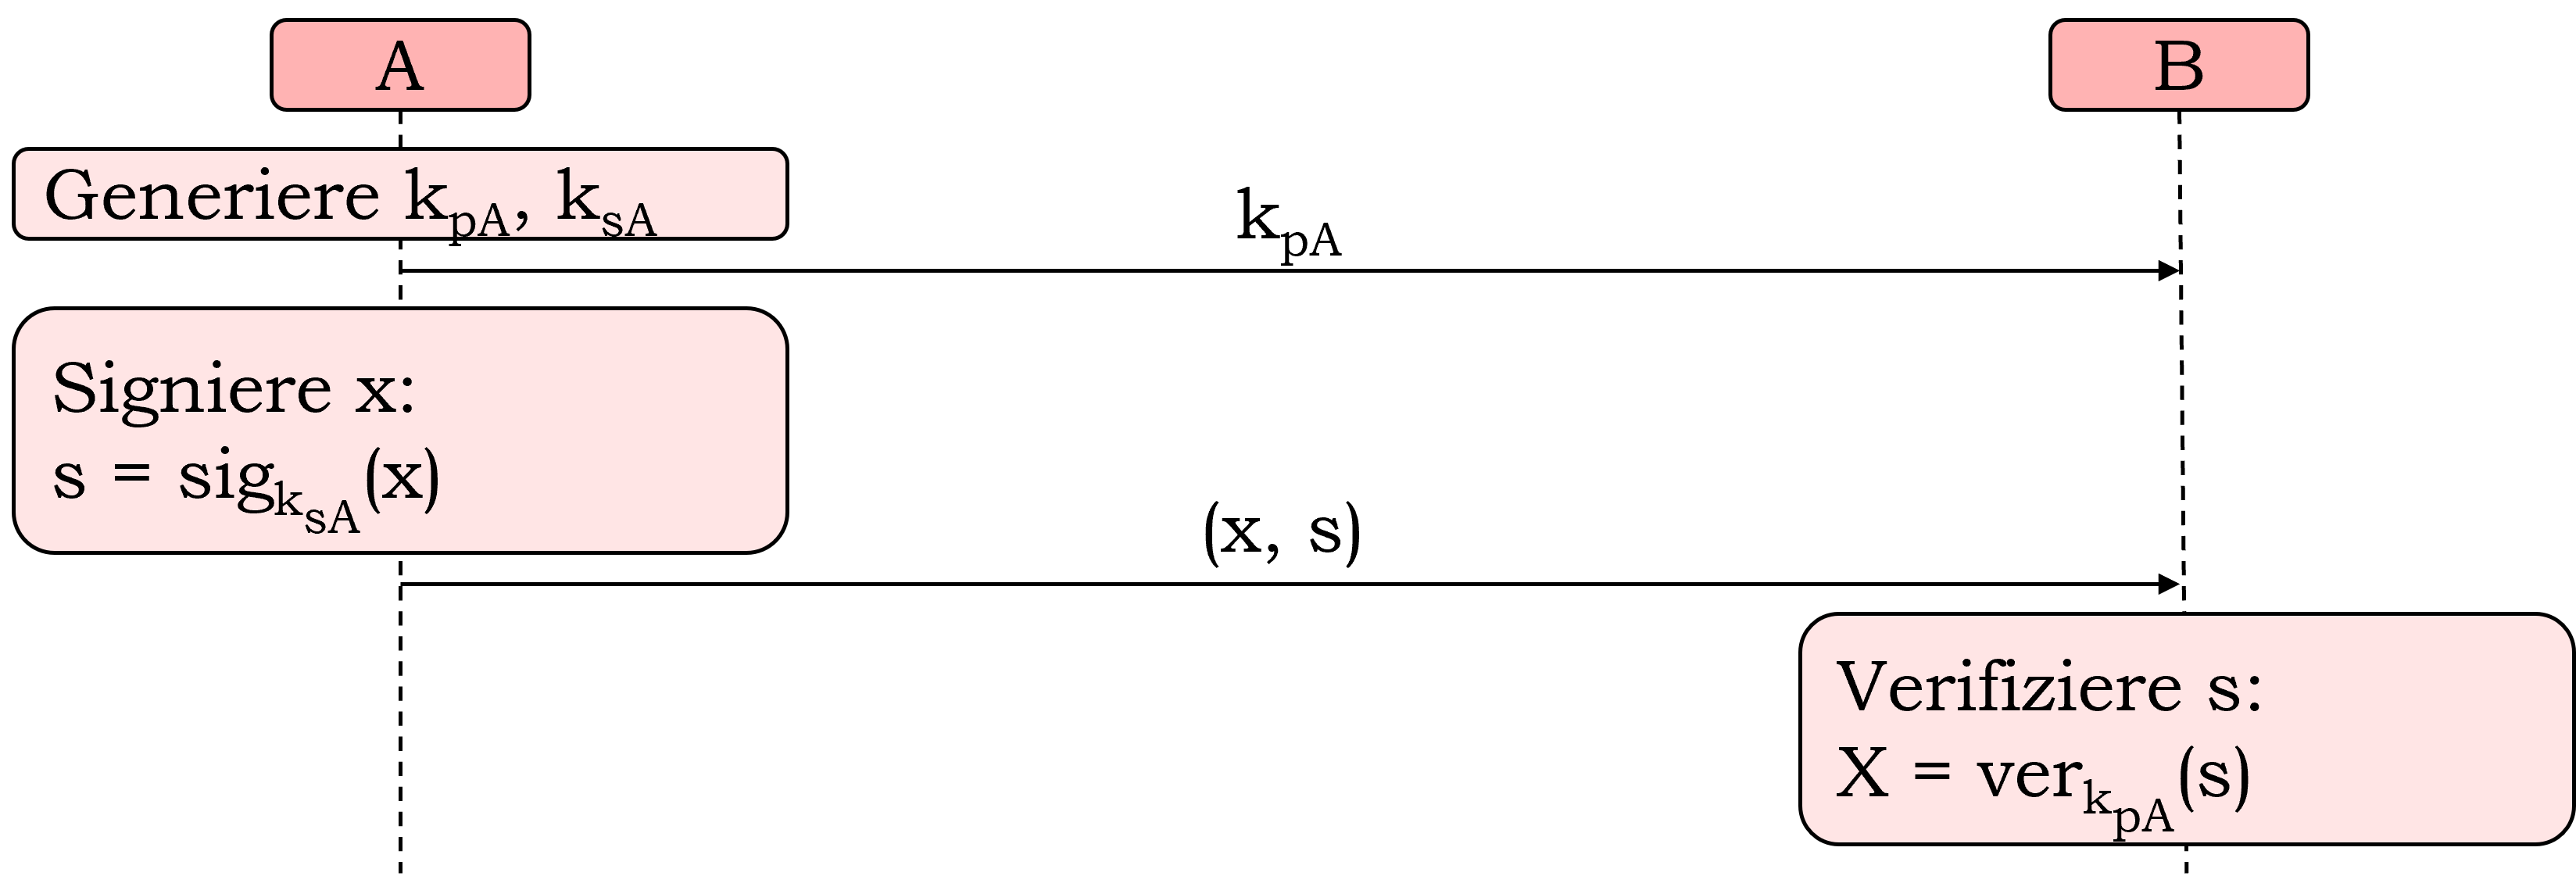
\includegraphics[width=\textwidth]{chapters/abb/grundlagen-sig}
				\caption{Ein einfaches Verfahren zur digitalen Signatur}
				\label{fig:grundlagen:sig}
			\end{figure}
			
			Das erste praktisch einsetzbare Verfahren zur digitalen Signatur wurde von Ronald Rivest, Adi Shamir und Len Adleman in einem Paper beschrieben. Dieses war jedoch noch nicht wirklich sicher, sondern zeigte lediglich, wie eine digitale Signatur prinzipiell umgesetzt werden könnte.\\
			
			Ein großes Problem von digitalen Signaturen ist, dass sichergestellt werden muss, dass der öffentliche Schlüssel auch wirklich zum Kommunikationspartner gehört. Dafür werden Zertifikate verwendet (vgl. Abschnitt \ref{subsec:grundlagen:krypto:cert}) \cite{Paar2010-E}.\\
			
			In den folgenden Abschnitten \ref{subsubsec:grundlagen:krypto:auth:rsa} bis \ref{subsec:grundlagen:krypto:auth:dsa} werden einige Authentifizierungsverfahren kurz vorgestellt.
			
			\subsubsection{RSA}
			\label{subsubsec:grundlagen:krypto:auth:rsa}
			
			RSA wird heute vor allem für das Verschlüsseln kleinerer Datenmengen (beispielsweise für den Transport kryptogrpahischer Schlüssel) und digitale Signaturen eingesetzt. Die Verschlüsselung mit RSA basiert auf dem Problem der Primfaktorzerlegung. Dies basiert darauf, dass es sehr effizient möglich ist, große Zahlen miteinander zu multiplizieren. Ein einfaches Faktorisierungsverfahren ist jedoch nicht bekannt.\\
			
			Die Funktionsweise von RSA wird in Abbildung \ref{fig:grundlagen:rsa} gezeigt.
			
			\begin{figure}[htbp]
				\centering
				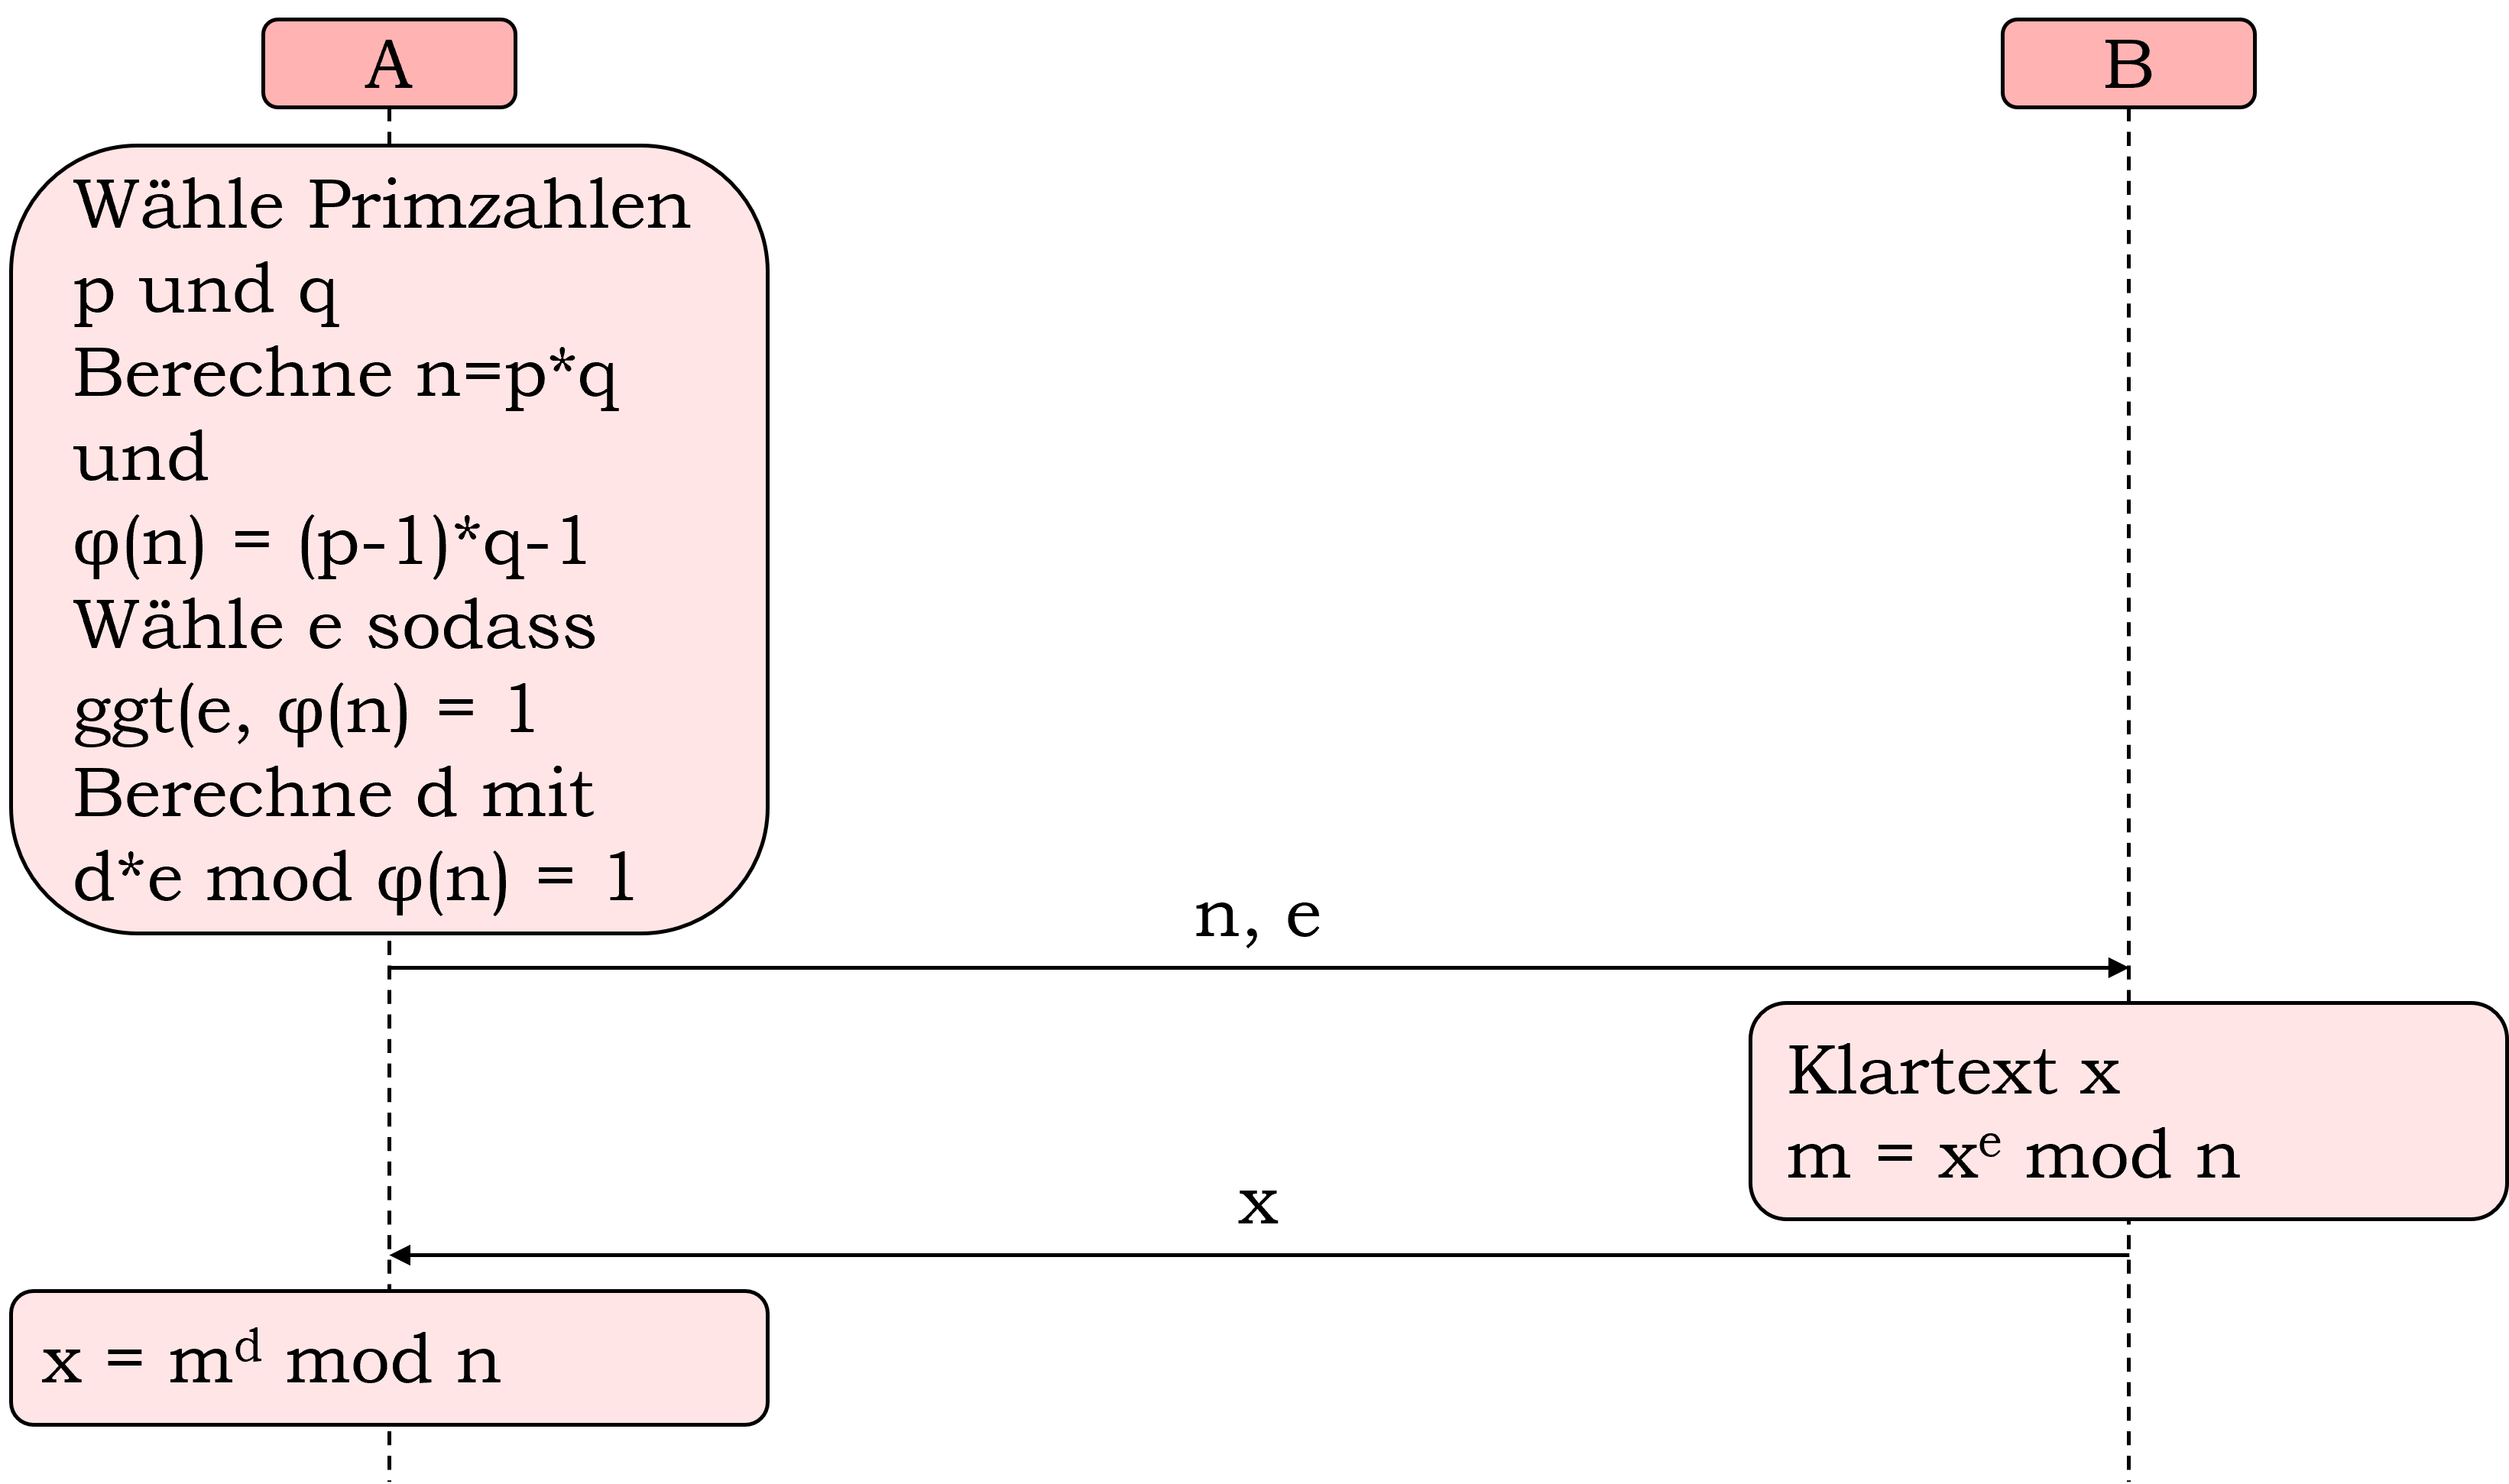
\includegraphics[width=\textwidth]{chapters/abb/grundlagen-rsa}
				\caption{Funktionsweise von RSA}
				\label{fig:grundlagen:rsa}
			\end{figure}
		
			RSA kann genauso zur digitalen Signatur verwendet werden. Dafür muss die gewünscht Nachricht mit dem privaten Schlüssel d signiert werden. Der Kommunikationspartner kann die Signatur dann mit dem öffentlichen Schlüssel e verifizieren.\\
			
			Dies ist aufgrund der Potenzregeln möglich:
			
			\[ (x^{e})^{d} = x^{ed} = x^{de} = (x^{d})^{e} \equiv h (\mod{n}) \]
			
			Die Sicherheit von RSA hängt dabei stark von der Länge der gewählten Primzahlen ab. 2020 war die größte öffentlich bekannte RSA-Zahl n, die faktorisiert werden konnte, 829 Bit lang. In der Praxis sind RSA-Schlüssel in der Regel zwischen 1024 und 4096 Bit lang. Aktuelle Empfehlungen sprechen sich für eine Schlüssellänge von mindestens 2048 Bit aus.\\
			
			RSA ist nur so lange sicher, wie es keinen effizienten Algorithmus zur Primzahlzerlegung gibt. Mit dem 1994 von Peter Shor vorgestellten Algorithmus ist dies, zumindest wenn man den Einsatz von Quantencomputern berücksichtigt, nicht mehr gegeben. Shors Algorithmus kann das Problem in Polynomialzeit lösen (vgl. Kapitel \ref{subsec:grundlagen:pqc:entwicklung}).
			
			\subsubsection{Rabin}
			\label{subsubsec:grundlagen:krypto:auth:rabin}
			
			Das Rabin-Kryptosystem ist eng mit RSA verwandt und basiert ebenfalls auf dem Faktorisierungsproblem. Dabei werden zur Schlüsselerzeugung folgende Berechnungen ausgeführt:
			
			\[ p\equiv3 \mod{4} \]
			\[ q\equiv3 \mod{4} \]
			\[ n=p*q \]
			
			Der öffentliche Schlüssel ist dann n. Der geheime Schlüssel ist (p, q).\\
			
			Um eine Nachricht zu verschlüsseln, muss diese zunächst auf einen Wert m < n abgebildet werden. Anschließend wird der Chiffretext c berechnet als $c=m^{2} \mod{n}$.\\
			
			Zur Entschlüsselung kann der chinesische Restsatz herangezogen werden, sofern p und q, die den geheimen Schlüssel bilden, bekannt sind. Dabei erhält man jedoch vier mögliche Klartexte. Welcher dieser vier möglichen Klartexte der richtige ist, muss erraten werden. Dies ist nur möglich, wenn der Klartext einer bestimmten Struktur (etwa einer Sprache) folgt. Ist dies nicht der Fall, muss eine solche Struktur künstlich erzeugt werden. Dies verringert jedoch die Sicherheit der Chiffre. Aus diesem Grund hat Rabin in der Praxis nur wenige Einsatzfelder.\\
			
			Auch digitale Signaturen können analog zu RSA durchgeführt werden.\\
			
			Anders als bei RSA kann für das Rabin-Kryptosystem bewiesen werden, dass die Schwierigkeit der Entschlüsselung genauso schwer ist wie das Faktorisierungsproblem selbst. Daher ist Rabin noch ein wenig sicherer als RSA.
			
			\subsubsection{Lamport-Einmal-Signaturverfahren}
			\label{subsubsec:grundlagen:krypto:auth:lamport}
			
			Ein weiterer Algorithmus, der zur digitalen Signatur verwendet werden kann, ist das Einmal-Signaturverfahren, das 1979 von Leslie Lamport entwickelt wurde. Für dieses wird eine Einmalfunktion - dies kann beispielsweise eine Hashfunktion sein - benötigt. Im folgenden Beispiel wird eine 256-Bit-Hashfunktion verwendet.\\
			
			Um den privaten Schlüssel zu generieren, müssen mit einem Zufallszahlengenerator 265 Paare von Zufallszahlen, d. h. insgesamt 512 Zufallszahlen, die jeweils eine Länge von 256 Bit haben, erzeugt werden. Für den zugehörigen öffentlichen Schlüssel werden die Hashwerte der 512 Zufallszahlen berechnet. Diese 512 Hashwerte sowie die verwendete Hashfunktion müssen veröffentlicht werden.\\
			
			Um nun eine Nachricht zu signieren, muss zunächst der Hashwert der Nachricht errechnet werden. Dieser hat per Definition 256 Bit. Für jede 0 in der gehashten Nachricht verschickt Alice nun die erste Zahl eines Zahlenpaars ihres geheimen Schlüssels, für jede 1 wählt sie die zweite Zahl des Zahlenpaares.\\
			
			Um die Signatur zu verifizieren, wird erneut der Hashwert der Nachricht errechnet. Außerdem müssen die Hashwerte der 265 Zufallszahlen des öffentlichen Schlüssels errechnet werden. Ist das erste Bit in der gehashten Nachricht eine 0, muss die erste Zahl des gehashten öffentlichen Schlüssels der ersten Zahl des ersten Zahlenpaares des öffentlichen Schlüssels entsprechen. Ist das erst Bit in der gehashten Nachricht eine 1, muss die zweite Zahl des ersten Zahlenpaares übereinstimmen.\\
			
			Da hier bei jedem Signaturvorgang die Hälfte des privaten Schlüssels veröffentlicht werden muss, kann mit jeden Schlüssel nur eine Signatur angefertigt werden. Danach ist der gesamte Schlüssel, d. h. auch die nicht verwendeten Zufallszahlen, zu löschen.\\
			
			Die Sicherheit dieses Signaturverfahrens basiert auf der Sicherheit der verwendeten Einwegfunktion. Wird hier eine schwache Funktion gewählt, so ist auch die Signatur nicht sicher. Wird hingegen eine starke Funktion gewählt, ist das Verfahren sehr sicher.\\
			
			Aktuell wird davon ausgegangen, dass das Lamport-Einmal-Signaturverfahren auch unter dem Einsatz von Quantencomputern noch sicher ist, solange eine große Hashfunktion verwendet wird.
			
			\subsubsection{Merkle}
			\label{subsubsec:grundlagen:krypto:auth:merkle}
			
			Digitale Signaturen mithilfe eines Merkle-Baums bauen auf dem Lamport-Einmal-Signaturverfahren auf. Sie ermöglichen jedoch eine endliche Anzahl an digitalen Signaturen mit demselben Schlüssel.\\
			
			Für dieses Verfahren wird ein Merkle-Baum benötigt (vgl. Abbildung \ref{fig:grundlagen:merkle}). Im Merkle-Baum ist jeder Knoten ein Hashwert der Verkettung seiner Kinder. Dies bedeutet beispielsweise:
			
			\[ a_{1,0} = H(a_{0,0}||a_{0,1}) \]
			\[ a_{2,0} = H(a_{1,0}||a_{1,1}) \]
			\[ a_{3,0} = H(a_{2,0}||a_{2,1}) \]
			
			\begin{figure}[htbp]
				\centering
				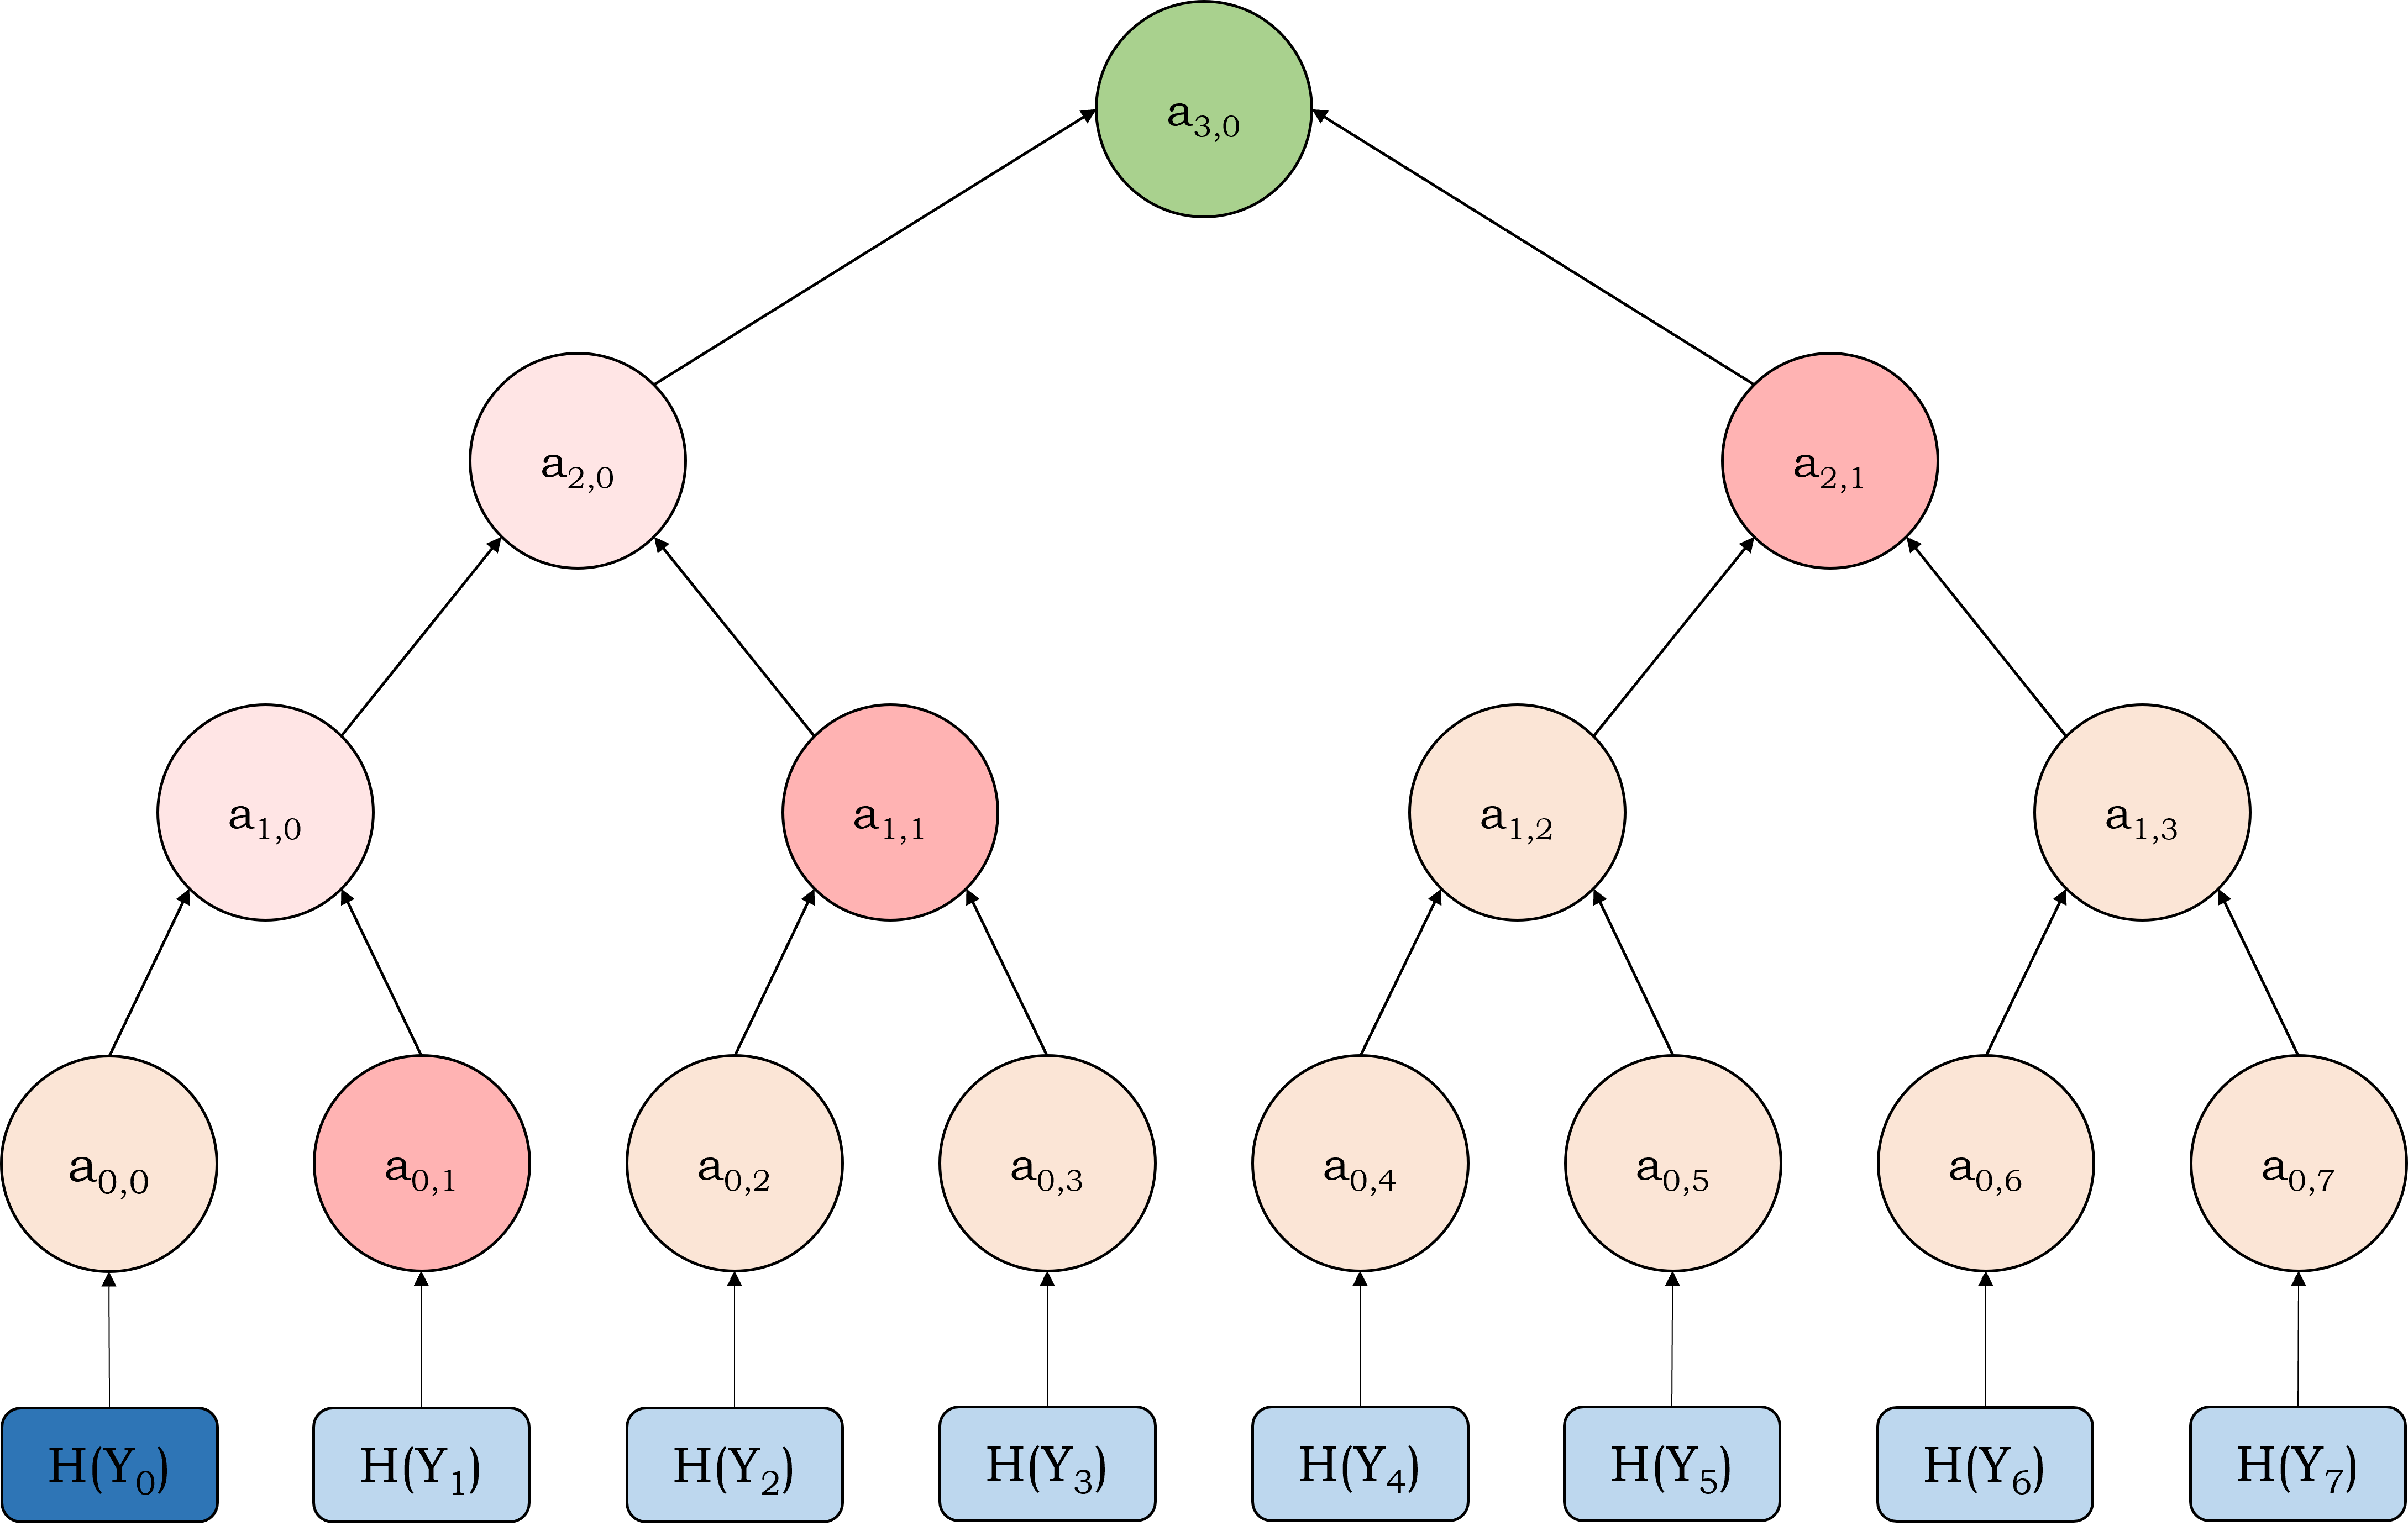
\includegraphics[width=\textwidth]{chapters/abb/grundlagen-merkle}
				\caption{Digitale Signaturen mithilfe eines Merkle-Baums}
				\label{fig:grundlagen:merkle}
			\end{figure}
		
			In der Abbildung ist beispielhaft ein Merkle-Baum für einen privaten Schlüssel aus acht Zufallszahlen dargestellt. Die einzelnen Zufallszahlen des Schlüssels Y\textsubscript{i} werden gehasht und bilden dann die Blätter des Merkle-Baums. Der öffentliche Schlüssel X ist die Wurzel des Baumes.\\
		
			Um nun eine Signatur prüfen zu können, wird nur eine Zufallszahl des geheimen Schlüssels benötigt. Zusätzlich müssen einige Knoten (in der Abbildung sind dies a\textsubscript{0,1}, a\textsubscript{1,1} und a\textsubscript{2,1}) zusätzlich übermittelt werden.
			
			
			
			\subsubsection{GMR}
			\label{subsubsec:grundlagen:krypto:auth:gmr}
			
			\subsubsection{DSA}
			\label{subsubsec:grundlagen:krypto:auth:dsa}
			
		\subsection{Kryptographische Zertifikate}
		\label{subsec:grundlagen:krypto:cert}
		
		Ein kryptographisches Zertifikat bindet einen öffentlichen Schlüssel an eine Entität. Dies kann eine natürliche Person oder auch eine Organisation oder ein System sein.\\
		
		Digitale Zertifikate enthalten in der Regel die folgenden Informationen:
		
		\begin{enumerate}
			\item den Namen des Ausstellers
			\item die Rahmenbedingungen unter denen das Zertifikat ausgestelle wurde
			\item die Gültigkeitsdauer des Zertifikats
			\item den öffentlichen Schlüssel des Eigentümers
			\item den Namen des Eigentümers
			\item ggf. weitere Informationen zum Eigentümer
			\item Zulässige Anwendungs- und Geltungsbereiche des Schlüssels
			\item eine digitale Signatur des Ausstellers über die o. g. Informationen
		\end{enumerate}
	
		Ein häufig verwendeter Standard für Zertifikate ist X.509. Dieser wird auch in TLS verwendet (vgl. Abschnitt \ref{sec:grundlagen:tls}).
	
	\section{Transport Layer Security}
	\label{sec:grundlagen:tls}
	
	TLS ist ein 1996 durch die \ac{IETF} festgelegtes Protokoll mit dem Ziel, einen Standard für die sichere Kommunikation im über das Internet zu finden. Das Protokoll agiert auf der Transportschicht. Während die ursprünglichen Ziele des Protokolls Datensicherheit und -integrität waren, wurde in späteren Versionen zunehmend auch die Kommunikation mit anderen TLS-Versionen sowie die Möglichkeit des Ausbaus des Protokolls, z. B. durch neue Algorithmen, betrachtet \cite{Kizza2020}.
	
	\section{Post-Quantum-Kryptographie und NIST}
	\label{sec:grundlagen:pqc}
	
		\subsection{Quanteninformatik}
		\label{subsec:grundlagen:pqc:quantencomputer}
	
		Während die klassische Einheit in der Informatik aus einem Bit entstehen kann, das entweder den Wert 0 oder den Wert 1 annehmen kann, wird die Grundlage der Quanteninformatik durch sogenannte Qubits gebildet. Diese unterscheiden sich in einigen wesentlichen Punkten von den klassischen Bits \cite{Just2020}:
		
		\begin{enumerate}
			\item Während der Wert eines klassischen Bits zu jedem Zeitpunkt eindeutig als 0 oder 1 identifiziert werden kann, können Qubits auch einen Wert zwischen 0 und 1 annehmen.
			\item Wird der Wert eines Qubits gemessen, ist dieser immer 0 oder 1. Der Wert eines Qubits kann sich demnach durch die Messung verändern.
			\item Eine Veränderung in einem Qubit kann eine instantane Veränderung in einem anderen Qubit hervorrufen.
		\end{enumerate}
	
		\subsection{Kryptoagilität}
		\label{subsec:grundlagen:pqc:agil}
		
		Ein wichtiges Konzept in diesem Zusammenhang ist das Konzept der Kryptoagilität. Durch die fortschreitende Entwicklung sind immer wieder etablierte kryptographische Verfahren unsicher geworden. Ist dies der Fall, müssen diese ersetzt werden.
	
		\subsection{National Institute of Standards and Technology}
		\label{subsec:grundlagen:pqc:nist}
		
		Das National Institute of Standards and Technology (übersetzt Nationales Institut für Standards und Technoligue) ist eine Bundesbehörde der Vereinigten Staaten, deren Hauptaufgabe Standardisierungsprozesse sind. In der Kryptographie war das NIST u. a. dafür verantwortlich, die Verschlüsselungsstandards \ac{AES} und \Ac{DES} zu standardisieren.
		
		\subsection{Entwicklung der Post-Quantum-Kryptographie}
		\label{subsec:grundlagen:pqc:entwicklung}
		
		\subsection{NIST-PQC-Verfahren}
		\label{subsec:grundlagen:pqc:verfahren}
		
			\subsubsection{Motivation}
			\label{subsubsec:grundlagen:pqc:verfahren:motivation}
			
			Das Internet basiert darauf, dass verschiedene Computersysteme miteinander interagieren können.
			Damit dies möglich ist, hat die internationale Gemeinschaft sich auf eine Reihe standardisierter Protokolle geeinigt.
			Einige dieser Protokolle sind durch die fortschreitende Entwicklung von Quantencomputern akut gefährdet.\\

			Ein Beispiel dafür ist RSA. RSA ist ein Algorithmus, der in vielen Protokollen verwendet wird.
			Er basiert auf dem Problem der Primfaktorzerlegung, d. h. darauf, dass es zwar leicht ist, große Zahlen zu multiplizieren, jedoch sehr schwer ist, eine große Zahl in ihre Primfaktoren zu zerteilen.
			Mit Shors Algorithmus, der auf Quantencomputern ausgeführt werden kann, ist dies jedoch effizient möglich \cite{Nist2016}.\\

			Auf der anderen Seite gibt es inzwischen eine große Anzahl an vorgeschlagenen Algorithmen, die diese Probleme lösen sollen.
			Um nun wieder geeignete Algorithmen zu finden, die sich für eine Standardisierung eignen, muss diese Menge an Algorithmen evaluiert werden.\\

			Dies soll durch das NIST-PQC-Verfahren umgesetzt werden.
			Ein ähnliches Verfahren wurde bereits von 1997 bis 2001 durchgeführt.
			Das Ergebnis des damaligen Verfahrens war die Standardisierung von AES \cite{Schneier2000}.\\
				
			\subsubsection{Verlauf}
			\label{subsubsec:grundlagen:pqc:verfahren:verlauf}
			
			\subsubsection{Status}
			\label{subsubsec:grundlagen:pqc:verfahren:status}
	
